%==============================================================================
% Sjabloon poster bachproef
%==============================================================================
% Gebaseerd op document class `a0poster' door Gerlinde Kettl en Matthias Weiser
% Aangepast voor gebruik aan HOGENT door Jens Buysse en Bert Van Vreckem

\documentclass[a0,portrait]{hogent-poster}

% Info over de opleiding
\course{Bachelorproef}
\studyprogramme{toegepaste informatica}
\academicyear{2022-2023}
\institution{Hogeschool Gent, Valentin Vaerwyckweg 1, 9000 Gent}

% Info over de bachelorproef
\title{Optimalisatie van de administratieve
workflow in juridische kantoren: auto-
matisering van repetitieve taken.}
\author{Duquesnoy Laurent}
\email{laurent.duquesnoy@student.hogent.be}
\supervisor{Jan Claes}
\cosupervisor{Stijn Dewolf (Deltalex)}

% Indien ingevuld, wordt deze informatie toegevoegd aan het einde van de
% abstract. Zet in commentaar als je dit niet wilt.
\specialisation{Mobile \& Enterprise Development}
\keywords{Automatisatie, repetitie, AI}

\begin{document}

\maketitle

\begin{abstract}
	Dit onderzoek richt zich op het verminderen van de administratieve werklast binnen advocatenkantoren door geautomatiseerde processen en integratie in de huidige software.
	Het omvat allereerst een analyse die bekijkt wat de specifieke bottlenecks zijn die repetitie bij advocaten veroorzaken en zo de productiviteit doen dalen.
	Dan wordt er onderzoek gevoerd naar tools die kunnen helpen bij het uitvoeren van deze taken of zelfs taken volledig kunnen overnemen.
	Daarna worden alle componenten samengevoegd en wordt er een stappenplan uitgetekend die de weg wijst naar een concrete RAG app.
	De voorgaande technische analyse zal een unieke kans zijn voor de onderzoeker om hun skills bij te scherpen op zowel het informaticadomein als in de administratieve/juridische sector.
\end{abstract}

\begin{multicols}{2} % This is how many columns your poster will be broken into, a portrait poster is generally split into 2 columns

	\section{Introductie}
	Deze bachelorproef handelt over het verbeteren van de efficiëntie van administratieve taken bij advocatenkantoren. 
    De natuur van de taken die deze beoogt te verbeteren zijn veelal repetitief in aard. Dit onderzoek ontspringt zich in de observatie
	dat bepaalde taken die uitgevoerd worden frustrerend en traag zijn. Een digitale
	assistent kan de tijd die deze taken innemen minimaliseren en het mogelijk maken
	deze te herinvesteren in taken die meer uitdagend en variërend zijn.

	\section{Conclusies}
	De uitkomst van deze bachelorproef is een uitgebreid technologisch onderzoek dat
	informatie bevat over iedere component van de opbouw van een digitale assistent.
	Eerst was de opzet van dit onderzoek om een assistent te implementeren en te
	integreren met bestaande software.
	Natuurlijk werkt deze assistent met libraries en componenten die toch heel wat
	resources gebruiken om vloeiend te bouwen, draaien en testen. Dit in combinatie
	met de gevoeligheid van de cliëntdata is de beslissing gekomen om dit onderzoek
	puur hypothetisch uit te voeren. Denk over dit onderzoek als een technologische
	gids om een lezer bekend te maken met de basisconcepten van Natural Language
	Processing, Large Language Models, Retrieval Augmented Generation en meer.
	Veel stappen uit dit onderzoek worden minder breed besproken gezien het hedendaagse aanbod van 
    digitale tools zoals JavaScript libraries, frameworks die al heel
	goeie implementaties voor digitale assistenten leveren en de extraordinaire snelle
	aard van verandering van het huidig technologisch spectrum.
	Er is in dit onderzoek geprobeerd om zo veel mogelijk technologiespecifiek te werken. 
    Het kan goed zijn dat er binnenkort betere technologieën uitgebracht worden
	die veel beter presteren dan degene die hier gebruikt worden. De technologieën
	gebruikt in dit onderzoek zijn op het moment van onderzoek de meest geschikte
	en performante op de markt, waarvan de meeste open-source.
	In conclusie hoop ik dat een lezer van dit onderzoek enerzijds bijleert over digitale
	assistenten en hoe ze werken onder de motorkap. Anderzijds dat hij het ook kan
	gebruiken als stappenplan tijdens het implementeren van zijn eigen assistent, iets
	waar de student die er nu aan werkt ook zeker gebruik van zal maken.

	\section{Toekomstig onderzoek}
	Dit onderzoek handelt over een topic die constant aan het evolueren is aan sneltreintempo.
	Als men deze proef gebruikt als een gids is het noodzakelijk dat er extra onderzoek gedaan wordt naar mogelijke upgrades, plaatsvervangers en documentatie van gebruikte technologieën.

\end{multicols}
\begin{figure}[h]
	\makebox[\textwidth]{
      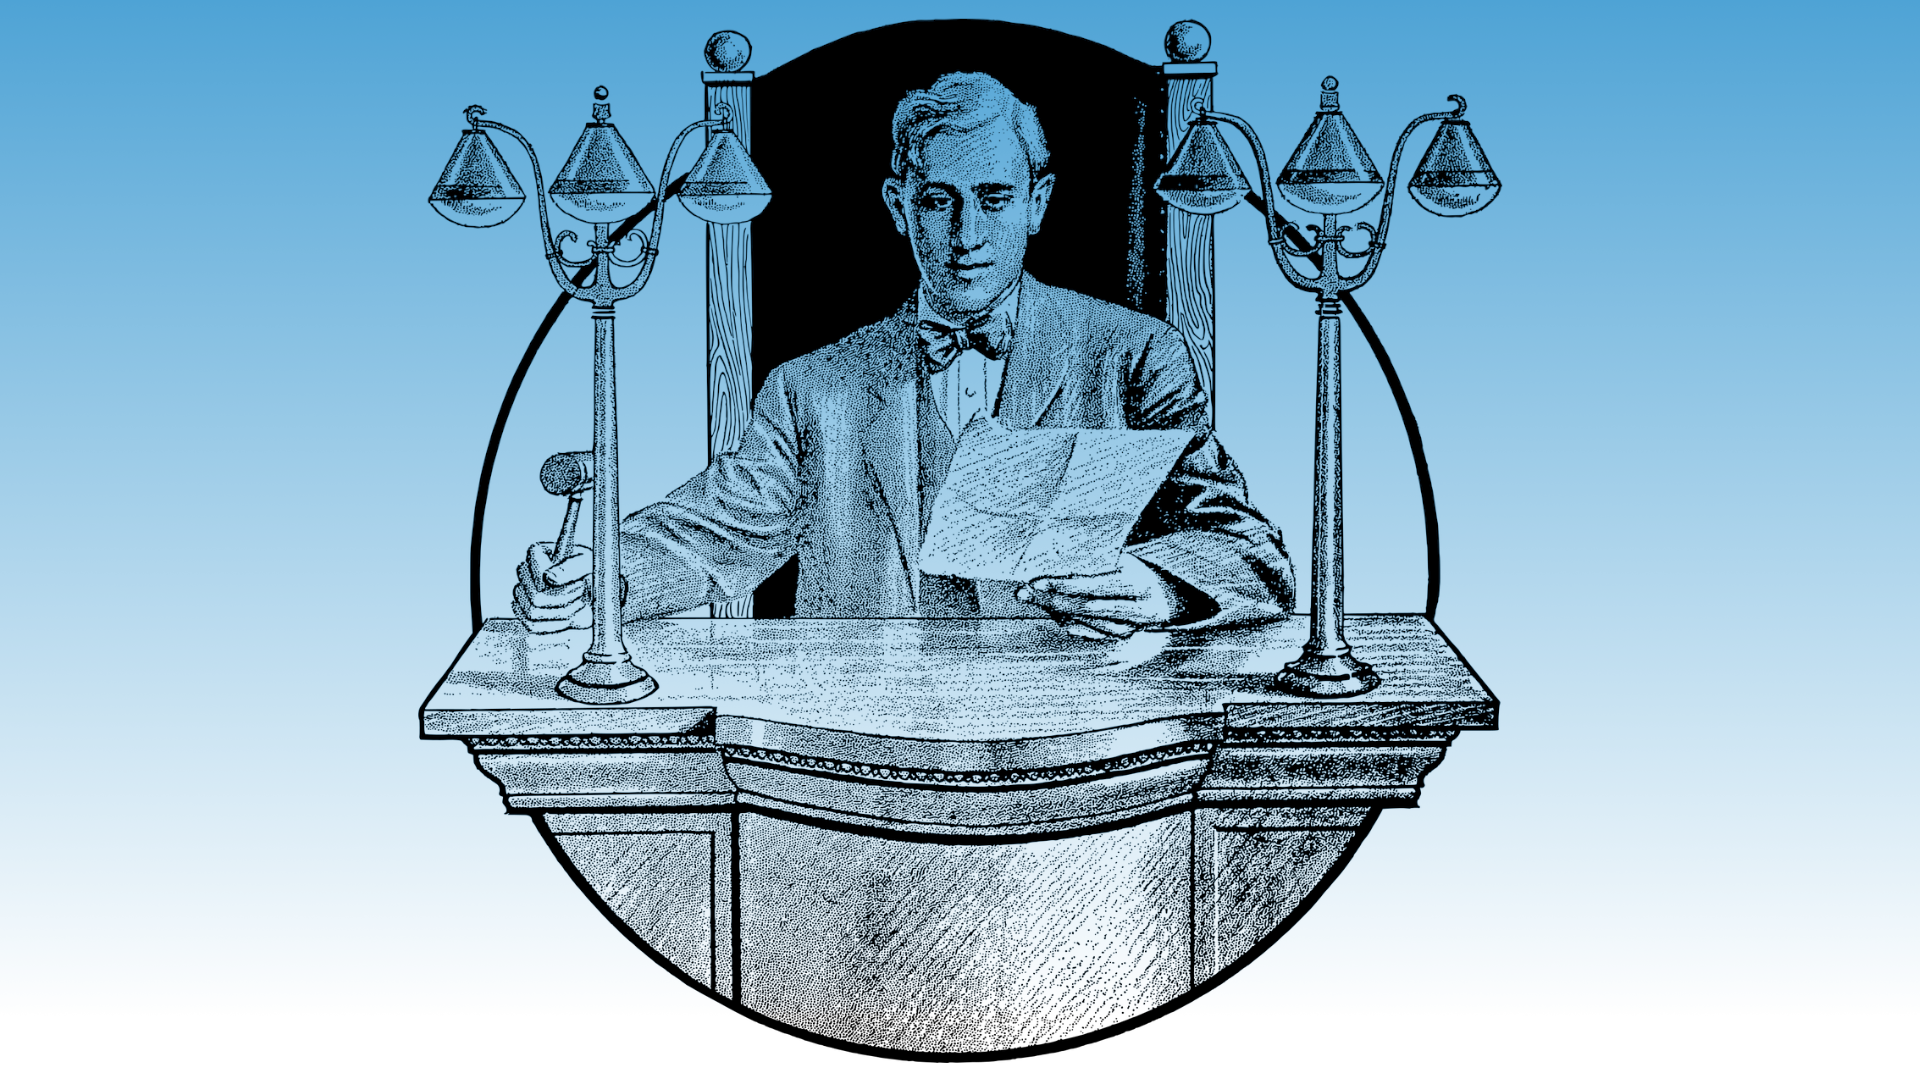
\includegraphics[width=\textwidth]{visual.png}

	}

	\captionof{figure}{Figuur 1: Ondersteunende visual (Judge by Gordon Johnson, Pixabay)}
\end{figure}



\end{document}
